The following example in Example~\ref{ex:heapcost} shows that in general 
resource cost analysis, the $\THESYSTEM$  can give a better cost upper bound than the traditional 
data-flow or control-flow analysis.
% program shown in Figure~\ref{fig:heapcost_example.tex} shows the similarity
% between the adaptivity and cost estimation.
\begin{example}[Nested While]
  \label{ex:whileNested}
The example program shown in Figure~\ref{fig:heap-nestedWhile} shows the similarity
between the adaptivity and cost estimation.

In order to estimate the worst case heap cost in this program, I analyse the length 
of the list assigned to $x$ and $y$ in line:6 and line : 9 of this program, through $\THESYSTEM$.
Then,  $\THESYSTEM$ computes approximation
of heap resource cost by searching for longest finite walk.
\\
Specifically as follows, 
$\THESYSTEM$ first constructs the program-based execution as in Figure~\ref{fig:heapcost_example.tex},
with weight on each vertex. (The query annotation in the graph is omitted, which isn't useful in analysing the 
list length).
Then $\THESYSTEM$ compute the longest restricted finite walk on this graph.
\\
In order to compute the bound for heap resource cost, the length of walk takes the non-query vertices into consideration as 
well. 

%  largest length of $x$ and $y$ 
% search for a path: $y^6 \to y^6$, and compute the adaptivity for this path as 
% $k$.
% Notice here, another special operation I have in the second branch is Non-updating of
% % Non-updating the 
% $\kw{querynum}$ and $\kw{flowcapacity}$.
% This guarantees both the accuracy and the soundness.
% Specifically,
% % because a second visiting of the same vertex 
% if this vertex is visited, it indicates that a cycle is monitored and  
% % indicates there is a cycle goes back to this vertex, 
% the traversing on this cycle is finished by going back to this vertex.
% %
% % then, when 
% When I continuously search for walks heading out of this vertex, 
% the minimum weight on this cycle does not affect the walks going out of this vertex that not pass this cycle.
% However, if I keep recording the minimum weight, then we
% %  are restricting 
% restrict the visiting times of vertices on a walk by
% using the minimum weight of vertices not on this walk.
% %  , it is unsound anymore.
% Then, it is obviously that this leads to unsoundness.
% If I update the $\kw{flowcapacity}[y^6]$ as $k$ after visiting $y^6$ the second time 
% on this walk,
% % the walk $y^6 \to y^6$,
% and continuously visit $x^9$,
% then the $\kw{flowcapacity[k]}$ is 
% updated as $\min(k, k^2)$.
% So
% %  which 
% % restricting 
% the visiting times of $x^9$ is restricted by $k$ on the walk $y^6 \to y^6 \to x^9$.
% This restriction excludes the finite walk $y^6 \to y^6 \to x^9 \to x^9$ where $y^6$ and $x^9$ visited by $k^2$ times
% in the computation. 
% However, the finite walk $y^6 \to y^6 \to x^9 \to x^9$ where $y^6$ is visited $k$ times and $x^9$ $k^2$ times is 
% a qualified walk, and exactly the longest walk I aim to find. So, by Non-updating the $\kw{flowcapacity}$ after 
% visiting $y$ again, I guarantee that the visiting times og vertices on every searched walk will not be restricted by weights not on this walk,
% i.e., the soundness.
% \\
% In the last line of this dfs algorithm, line: 16, it returns the adaptivity heading out from its input vertex.
% \\
% By applying this deep first search strategy on every vertex on this SCC, 
% I compute the adaptivity of this SCC by taking the maximum 
% % adaptivity reaching every vertex on this SCC.
% value over every vertex.
%
As a result,
the largest heap resource consumed in total, by $y$ and $x$ together computed from the $\THESYSTEM$ is $1 + k^2 + k$.
Comparing to $k + k^2 + k^3$ estimated as  the longest weight path from traditional CFL-reachability method, 
$\THESYSTEM$ analysis result improves the accuracy by $O(n)$.

% Look at a Nested While Loop example program in Figure~\ref{fig:heapcost_example.tex}.
% Specifically,
% % because a second visiting of the same vertex 
% if this vertex is visited, it indicates that a cycle is monitored and  
% % indicates there is a cycle goes back to this vertex, 
% the traversing on this cycle is finished by going back to this vertex.
% %
% % then, when 
% When I continuously search for walks heading out of this vertex, 
% the minimum weight on this cycle does not affect the walks going out of this vertex that not pass this cycle.
% However, if I keep recording the minimum weight, then we
% %  are restricting 
% restrict the visiting times of vertices on a walk by
%  using the minimum weight of vertices not on this walk.
% %  , it is unsound anymore.
% Then, it is obviously that this leads to unsoundness.
 %
  %
  \begin{figure}
    \centering
    {
      % \footnotesize
    \begin{subfigure}{.4\textwidth}
    \begin{centering}
    % 
    $ 
    \begin{array}{l}
      \kw{whileNested}(k) \triangleq \\
      \clabel{\assign{i}{k} }^{0} ; 
      \clabel{ \assign{x}{[]}}^{1} ; 
      \clabel{ \assign{y}{[]}}^{2} ; \\
          \ewhile ~ \clabel{i > 0}^{3} ~ \edo ~ \\
          \Big(
           \clabel{\assign{i}{i-1}}^{4} ;
           \clabel{\assign{j}{k}}^{5} ;\\
           \clabel{\assign{x}{1::y} }^{6}  ; \\
           \ewhile ~ \clabel{j > 0}^{7} ~ \edo ~ \\
           \Big(
            \clabel{\assign{j}{j-1}}^{8};
            \clabel{\assign{y}{ 1::x }}^{9}
            \Big) \Big)
      \end{array}
    %       
    $
    \caption{}
    \end{centering}
    \end{subfigure}
    \quad
    \begin{subfigure}{.52\textwidth}
      \begin{centering}
      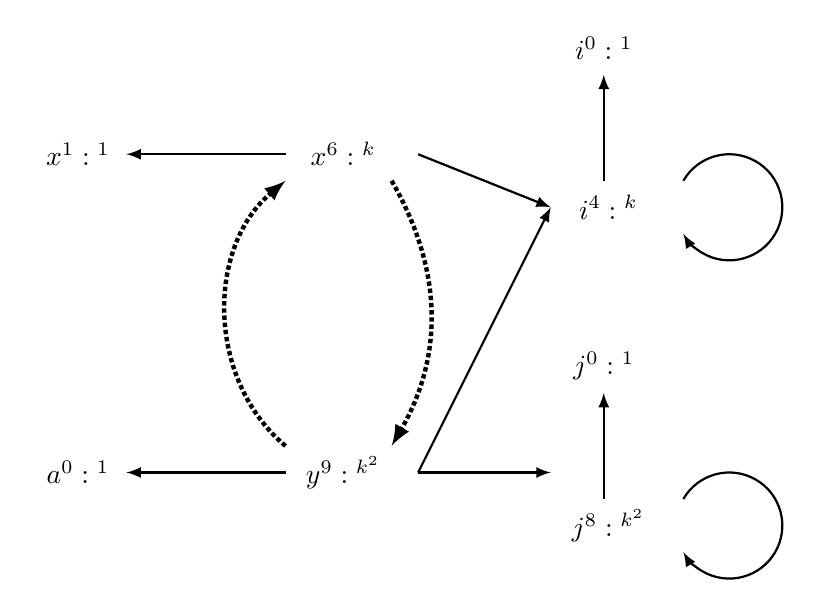
\begin{tikzpicture}[scale=\textwidth/18cm,samples=200]
      % Variables Initialization
      \draw[] (-5, 1) circle (0pt) node{{ $a^0: {}^1$}};
      \draw[] (-5, 7) circle (0pt) node{{ $x^1: {}^{1}$}};
      % Variables Inside the Loop
      \draw[] (0, 7) circle (0pt) node{{ $x^6: {}^{k}$}};
      \draw[] (0, 1) circle (0pt) node{{ $y^9: {}^{k^2}$}};
      % Counter Variables
      \draw[] (5, 9) circle (0pt) node {{$i^0: {}^{1}$}};
      \draw[] (5, 6) circle (0pt) node {{ $i^4: {}^{k}$}};
      \draw[] (5, 3) circle (0pt) node {{$j^0: {}^{1}$}};
      \draw[] (5, 0) circle (0pt) node {{ $j^8: {}^{k^2}$}};
      % Value Dependency Edges:
      \draw[ thick, -latex] (5, 6.5)  --       (5, 8.5) ;
      \draw[ thick, -latex] (5, 0.5)  --       (5, 2.5) ;
      % Value Dependency Edges on Initial Values:
      \draw[ thick, -latex,] (-1, 1)  -- (-4, 1) ;
      \draw[ thick, -latex,] (-1, 7)  -- (-4, 7) ;
      %
      \draw[ ultra thick, -latex, densely dotted,] (-1, 1.5)  to  [out=-220,in=220]  (-1, 6.5);
      % node[left]{\highlight{{$k$}}}
      \draw[ ultra thick, -latex, densely dotted,]  (1, 6.5) to  [out=-60,in=60] (1, 1.5) ;
      % node[right]{\highlight{{$k$}}}
      % Control Dependency
      \draw[ thick, -latex, ] (6.5, 6.5) arc (150:-150:1);
      \draw[ thick, -latex, ] (6.5, 0.5) arc (150:-150:1);
      \draw[ thick,-latex] (1.5, 7)  -- (4, 6) ;
      \draw[ thick,-latex] (1.5, 1)  -- (4, 6) ;
      \draw[ thick,-latex] (1.5, 1)  -- (4, 1) ;
   \end{tikzpicture}
   \caption{}
      \end{centering}
      \end{subfigure}
    }
     \caption{(a) Nested While Loop Example, (b) Execution-Based Dependency Graph, (c) The Static Program-Based Dependency graph.}
    \label{fig:whileSim}
    \vspace{-0.5cm}
    \end{figure}
  \end{example}
